\documentclass[a4paper,parskip=half]{scrartcl}

\usepackage[T1]{fontenc}
\usepackage[ngerman]{babel}
\usepackage{csquotes}
\usepackage[regular,condensed,sfdefault]{roboto}
\usepackage{graphicx}
\usepackage{chemformula}
\usepackage[backend=biber]{biblatex}
\usepackage[hidelinks,pdfencoding=auto,
  pdfauthor={Thomas Ascher},
  pdfusetitle,
  pdfkeywords={Bier,Kegging,Zapfanlage}]{hyperref}
\usepackage{microtype}

\addto\extrasngerman{
\def\figureautorefname{Abb.}
}

\addto\captionsngerman{
\renewcommand{\figurename}{Abb.}
}

\title{Kegging: Ein Kurzüberblick}
\author{Thomas Ascher}

\addbibresource{kegging.bib}

\begin{document}
\maketitle

\section*{Einleitung}

Besteht Interesse daran, das eigene Bier mit amtlicher Schaumkrone selbst zu zapfen, größere Sude mit vertretbarem Zeitaufwand abzufüllen oder der Sisyphusarbeit der Flaschenreinigung zu entrinnen, ist die Anschaffung von Fässern bzw. Kegs und der dazu passenden Zapfanlage der nächste unausweichliche Schritt. Dieser erfordert jedoch u. a. die Auseinandersetzung mit physikalischen Effekten, neuen Gerätschaften und verschiedenen Gewindenormen \autocite{GastroBrennecke2021}. Der vorliegende Artikel soll hierbei Hilfestellung leisten.

\textbf{Achtung}: Die in Zapfanlagen eingesetzten Gase können in hohen Konzentrationen zum Erstickungstod führen. Druckgasbehälter stehen unter hohem Druck. Es ist dementsprechend für eine sichere Aufstellung zu sorgen. Ein maximal zulässiger Betriebsdruck sollte nicht überschritten werden, da dies Anlagen- und Personenschäden zur Folge haben kann.

\section*{Weg von der Flasche?}

Abgesehen von langen Reinigungs- und Abfüllzeiten bieten Flaschen viele Vorteile: breite Verfügbarkeit, kostengünstige Anschaffung und einfache Handhabung. Zudem sind sie in kleiner Stückzahl leicht zu transportieren und in einem Kühlschrank zu verstauen. Warum also stattdessen Kegs als Gebinde nutzen? Abgesehen von einer höheren strukturellen Stabilität sind auch eine bessere Handhabbarkeit der Karbonisierung und die Möglichkeit der sauerstoffarmen Abfüllung Gründe dafür. Mit welchen Kosten wäre also bei einem Umstieg zu
rechnen? Mittlerweile existieren verschiedene Lösungen im Heimbraubereich. Das
Angebot reicht von Mini Keg Komplettsystemen, wie sie z. B. iKegger ab rund
€ 130 im Sortiment hat, bis hin zu Zapfkühlschränken mit mehreren Zapfhähnen,
die mit allen dazugehörigen Komponenten eher im Bereich von über € 1000 liegen.
Selbst gebaute Systeme mit gebrauchten Komponenten sind entsprechend günstiger.

\section*{Aufbau und Funktionsweise einer Zapfanlage}

Eine Zapfanlage besteht aus vielen Einzelkomponenten \autocite{BrewersAssociation2019}. Das sind u. a. Kühlsysteme, Kegs, Druckgasbehälter mit Zapfgas, Druckminderer, Bier-/Gasleitungen, Zapfköpfe, Schanksäulen, Zapfhähne, Durchgangsstutzen, Distanzhülsen, Verteiler, Schlauchtüllen, Schellen, Verbinder und Kupplungen. Die trivialste Form (\autoref{fig:zapfanlage}) eines solchen Aufbaus ist ein Keg, an das eine Gasquelle in der Form einer Gaspatrone und eine Zapfarmatur in der Form eines Picknick-Zapfhahns aufgesteckt werden \autocite{Westemeier1995}.

\begin{figure}[h]
\centering
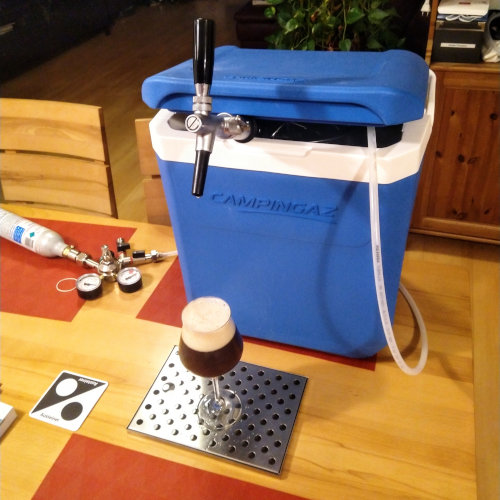
\includegraphics[width=5cm]{images/zapfanlage.jpg}
\caption{Einfache NC Zapfanlage}
\label{fig:zapfanlage}
\end{figure}

Von der Systematik her drückt in einer Zapfanlage Gas aus einem Druckgasbehälter, geregelt über einen Druckminderer, Bier aus einem Keg über Leitungen bis hin zu einem Zapfhahn. Dieser Vorgang muss bei passendem Betriebsdruck und passender Durchflussrate erfolgen, da es beim Ausschank sonst zu einer übermäßigen Schaumbildung kommt. Als Zapfgas wird primär Kohlendioxid (\ch{CO2}) oder ein Gemisch aus Kohlendioxid und Stickstoff (\ch{N2}) eingesetzt. Anders als Kohlendioxid löst sich Stickstoff nicht so leicht in Bier. Dieser Effekt lässt sich dazu nutzen, um bei einem ungünstigen Betriebsdruck die Karbonisierung des zu zapfenden Biers konstant zu halten. \autocite{BrewersAssociation2019} Gase für den Schankbetrieb sind z. B. als Flaschengas bei Linde Gas zu beziehen. Mini Keg Systeme sind alternativ auch durch Gaspatronen oder mit entsprechendem Adapter durch SodaStream Flaschen zu betreiben.

Flaschengas steht unter hohem Druck. Die Überführung in einen gewünschten Ausgangsdruck erfolgt mittels Druckminderer (\autoref{fig:druckminderer}). Dieser besteht aus einem genormten Gasflaschenanschluss, ein bis zwei Manometern, einer Einstellschraube und mindestens einem Gasauslass. Das Manometer gegenüber dem Flaschenanschluss zeigt üblicherweise den Flaschendruck an, das Manometer gegenüber dem Gasauslass den Betriebsdruck. Durch den Einbau weiterer Zwischendruckminderer ist es möglich, mehrere Leitungen mit unterschiedlichem Betriebsdruck aus der gleichen Gasflasche zu betreiben. Hierbei muss der Hauptdruckminderer um circa 0,35 bis 0,7 Bar höher eingestellt werden als die höchste Einstellung der Zwischendruckminderer. \autocite{BrewersAssociation2019}

\begin{figure}[h]
\centering
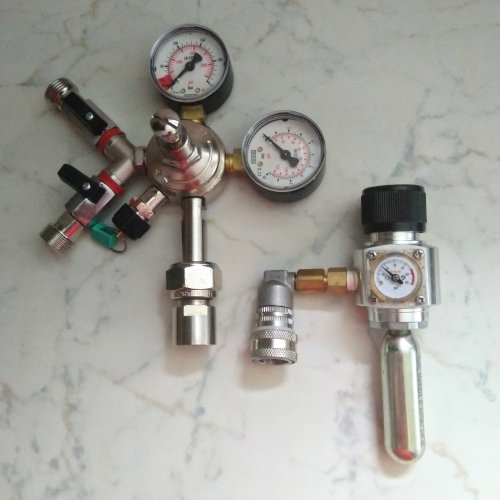
\includegraphics[width=4.8cm]{images/druckminderer.jpg}
\caption{Druckminderer}
\label{fig:druckminderer}
\end{figure}

Zapfhähne existieren in verschiedenen Bauarten, die zum Teil zusätzliche Funktionen wie eine Schaumtaste oder einen Kompensator integriert haben. Per Kompensator (\autoref{fig:kompensatorhahn}) lässt sich durch einen Einstellhebel die Durchflussrate regulieren und somit ein zu hoher Betriebsdruck ausgleichen. Das ermöglicht das Zapfen von Bieren mit unterschiedlicher Karbonisierung bei gleicher Leitungslänge. Der Anschluss eines Zapfhahns erfolgt an einen Stutzen mithilfe eines speziell dafür vorgesehen Zapfhahn-Schlüssels. Schlauchverbindungen werden dann entweder mittels Schlauchtülle, Nippel oder Steckverbindungen, wie das John Guest DMfit oder Kegland Duotight System, eingerichtet.

\begin{figure}[h]
\centering
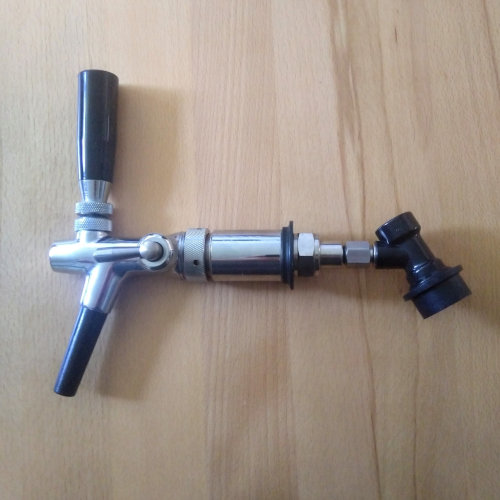
\includegraphics[width=4.8cm]{images/kompensatorhahn.jpg}
\caption{Kompensatorhahn mit NC Kupplung}
\label{fig:kompensatorhahn}
\end{figure}

\section*{Kegtypen}

In der Gastronomie haben sich mehrere Systeme \autocite{HWBS2021} für den Ausschank etabliert, von denen im Heimbraubereich insbesondere die für Soda konzipierten Cornelius/Corny Kegs und die für Bier konzipierten Euro/DIN/Slim/Sankey Kegs Anwendung finden.

\begin{figure}[h]
\centering
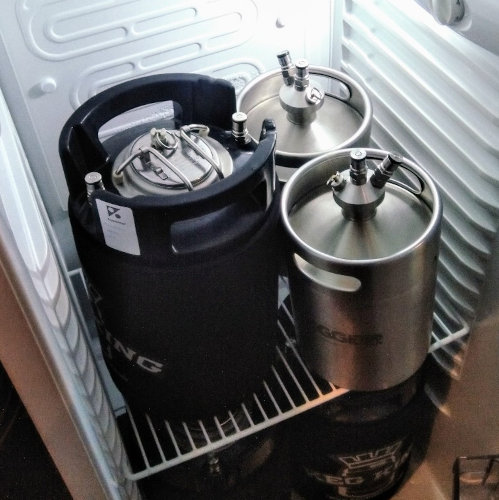
\includegraphics[width=4.8cm]{images/keg.jpg}
\caption{NC Kegs}
\label{fig:keg}
\end{figure}

Cornelius Kegs existieren für Abfüllvolumen von 2 bis 18 Liter als zwei verschiedene Typen: Non Coke (CC) mit Ball Lock (\autoref{fig:keg}) und Coca-Cola (CC) mit Pin Lock \autocite{Westemeier1995}. Die CC Variante ist ein Auslaufmodell \autocite{Gretzschel2016}. Der Anschluss von Soda Kegs erfolgt über Kupplungen. Das sind bei NC Kegs eine schwarze Steckkupplung für die Bierleitung und eine Graue für die Gasleitung (\autoref{fig:kupplungen}). Das Ventil für Gas ist zur besseren Erkennung mit einer Kerbe markiert. Beide Kupplungen haben zwar einen unterschiedlichen Innendurchmesser, lassen sich aber mit dem entsprechenden Kraftaufwand falsch aufstecken. Schraubverbindungen des NC Systems haben ein 7/16“ UNF Gewinde. Gaskupplungen sind auch mit integriertem Rückschlagventil erwerbbar. Dieses verhindert einen Einlauf von Bier in die angeschlossene Gasleitung und schützt somit den nächsten Druckminderer vor Beschädigungen.

\begin{figure}[h]
\centering
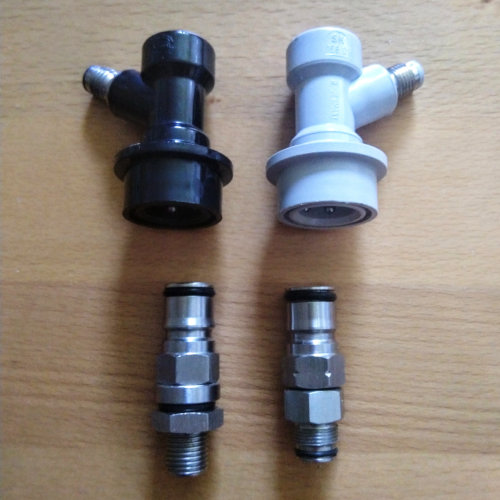
\includegraphics[width=4.8cm]{images/kupplungen.jpg}
\caption{NC Kupplungen}
\label{fig:kupplungen}
\end{figure}

Die von Brauereien eingesetzten Euro Kegs sind auf einen Betriebsdruck von 3 bis 7 Bar ausgelegt und für Abfüllvolumen von 5 bis 50 Liter verfügbar. Anschlusssysteme existieren in mehreren inkompatiblen Varianten. Das sind in Österreich zumindest Flach Fitting (Typ A), Kombi Fitting (Typ M) und Korb Fitting (Typ S). Je nach Keg variiert auch noch das Gewinde zum Einschrauben des Steigrohrs. \autocite{HWBS2021a} Der Anschluss eines Euro Kegs erfolgt über einen Zapfkopf, der je nach Typ entweder aufgeschoben oder aufgesteckt und danach mit einem Hebel arretiert wird. Bierleitungen werden per Überwurfmutter an 5/8“ Gewinde entweder vertikal (Kelleranstich) oder horizontal (Thekenanstich) angeschraubt, Gasleitungen typischerweise an ein 3/4“ Gewinde.

Für welchen Kegtyp man sich letztendlich entscheidet, ist Geschmackssache. Die Vorteile von Euro Kegs und weiteren Varianten sind eine vermutlich höhere Komponentenlebensdauer, die Kompatibilität mit Gastroanlagen und die Verfügbarkeit von Fassgrößen bis 50 Liter. Für Cornelius Kegs sprechen geringere Neuanschaffungskosten, ein entfernbarer Deckel zur besseren Reinigung und die Handhabung ohne Spezialwerkzeug. Während Euro Kegs meist mit einer Berstscheibe als Überdruckschutz ausgerüstet sind, besitzen Cornelius Kegs ein Überdruckventil, welches auch der Kegentlüftung dient.

\section*{Abfüllung und Karbonisierung}

Kegs lassen sich einfach und schnell per Schlauch aus einem Gärbehälter befüllen (\autoref{fig:transfer}). Eine Waage ermöglicht dabei die Messung des Füllfortschritts. Zur Minimierung der Sauerstoffaufnahme während des Transfers kann ein Keg vorab mit \ch{CO2} geflutet (vorgespannt) werden. Dies ist durch mehrere Methoden zu bewerkstelligen: Keg mit Flüssigkeit befüllen und diese mit Zapfgas wieder herausdrücken oder Zapfgas am Boden eines leeren Kegs einleiten, um somit eine Gasdecke zu bilden.

\begin{figure}[h]
\centering
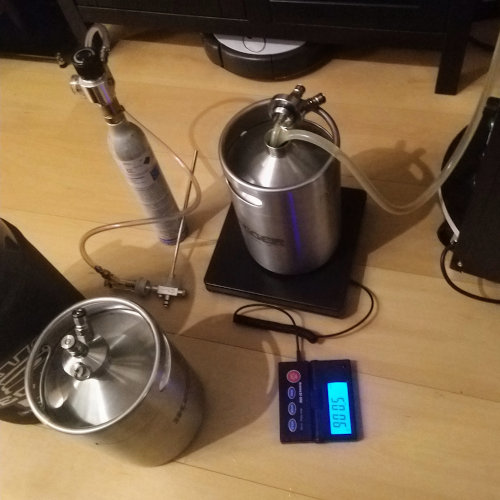
\includegraphics[width=4.8cm]{images/transfer.jpg}
\caption{Umschlauchen aus Gärbehälter}
\label{fig:transfer}
\end{figure}

Druck-Gärbehälter, wie z. B. der FermZilla Allrounder, unterstützen eine direkte Verbindung zu einem NC Keg und ermöglichen somit einen geschlossenen Transfer mit minimalem Sauerstoffkontakt (\autoref{fig:geschlossenertransfer}). Ein Spundventil am Gaseingang des Zielkegs erlaubt dabei eine gewisse Regelung der Durchflussrate. Ein Umdrücken von ungekühltem Bier ist zu vermeiden, da der dabei entstehende Schaum mitunter zu einer Leitungsverstopfung führt.

\begin{figure}[h]
\centering
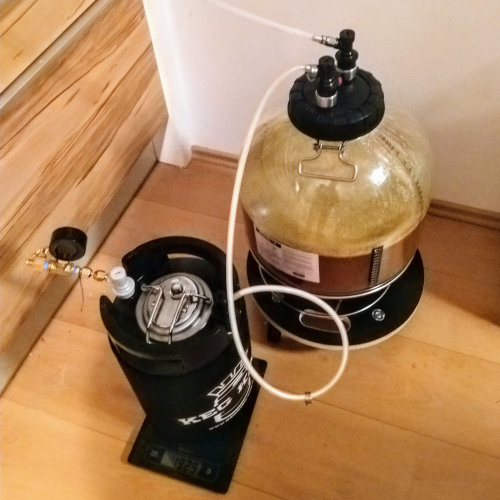
\includegraphics[width=4.8cm]{images/geschlossener_transfer.jpg}
\caption{Geschlossener Transfer aus Druck-Gärbehälter}
\label{fig:geschlossenertransfer}
\end{figure}

Bezüglich der Karbonisierung ist ein Keg wie eine große Flasche zu betrachten. Alle Methoden der Flaschengärung sind dementsprechend anwendbar. Dabei ist zu beachten, dass die für Flaschen veranschlagte Zucker-/Speisegabe je nach Füllstand angepasst werden muss. Bei einem vollgefüllten Keg ist diese circa um die Hälfte zu reduzieren. Zur Sicherstellung, dass der Klemm-Deckel eines Cornelius Kegs korrekt dichtet, sollte nach dem Verschließen des Deckels mit \ch{CO2} ein wenig Druck im Keg aufgebaut werden. Während der Karbonisierung erlaubt ein Spundventil mit Manometer (\autoref{fig:spundventil}) eine Kontrolle und Korrektur des Drucks im Keg.

\begin{figure}[h]
\centering
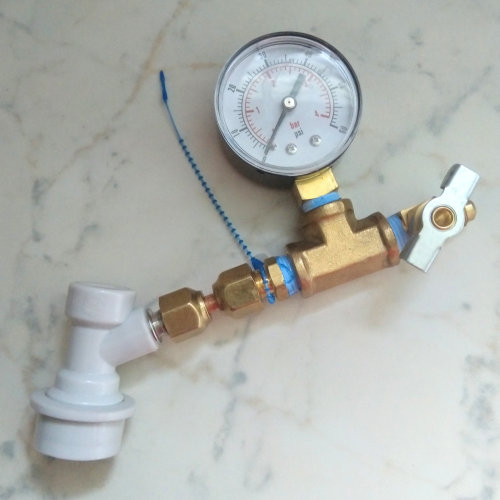
\includegraphics[width=4.8cm]{images/spundventil.jpg}
\caption{Spundventil mit NC Kupplung}
\label{fig:spundventil}
\end{figure}

Zusätzlich zur natürlichen Karbonisierung lässt sich eine gewünschte Karbonisierung auch durch Zwangskarbonisierung mit \ch{CO2} Einleitung einstellen \autocite{Sparks}. Dabei muss basierend auf Umgebungstemperatur, Umgebungsdruck und Alkoholgehalt eines Biers ein passender Sättigungsdruck am Druckminderer gewählt werden. Eine Änderung an einem dieser Parameter erfordert demnach eine Druckanpassung. Hierbei gilt, je geringer die Umgebungstemperatur ist, desto weniger Druck wird benötigt, damit \ch{CO2} in Lösung geht. Die Bestimmung des korrekten Sättigungsdrucks erfolgt über Spundungs-/Karbonisierungstabellen oder durch Apps, wie dem „EasyBlend Calculator“ (\autoref{fig:mcdantim}) von McDantim \autocite{McDantim2021}. Je nach Software ist die Karbonisierung entweder in Gramm von \ch{CO2} pro Liter Bier (g/l), Vol \% oder Volumen von \ch{CO2} (vols) zu spezifizieren. Mit Volumen ist hierbei ein Vielfaches des zu karbonisierenden Behältervolumens gemeint. Ein g/l entspricht ungefähr 0,5 vols \autocite{BrewersAssociation2019}.

\begin{figure}[h]
\centering
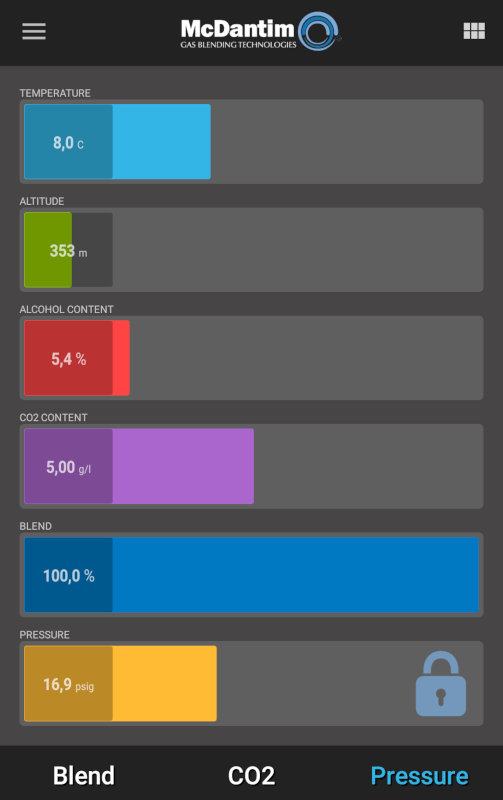
\includegraphics[width=4.8cm]{images/mcdantim.jpg}
\caption{EasyBlend Calculator}
\label{fig:mcdantim}
\end{figure}

Es dauert mehrere Tage, bis eine gewünschte \ch{CO2} Menge bei passendem Sättigungsdruck in Lösung geht. Diese Zeitspanne ist durch zwei weniger deterministischen Methoden zu beschleunigen: einen höheren Sättigungsdruck für einen kürzeren Intervall einzustellen oder ein Keg bei der Karbonisierung zu bewegen, um die Oberflächenspannung des Biers zu durchbrechen, was eine schnellere Gasaufnahme bewirkt. Je größer die Kontaktfläche, desto mehr Gas kann in der gleichen Zeit in Lösung gehen. Ein NC Keg kann hierfür gekühlt am Boden in horizontale Lage gebracht und mit dem Fuß leicht vor und zurück gerollt werden. Solange eine Gasaufnahme erfolgt, ist ein Zischen im Druckminderer wahrzunehmen. Variante zwei kann jedoch bei Flüssigkeitseintritt in die Gasleitung Beschädigungen am Druckminderer zufolge haben.

\section*{Ausschank}

Für einen Zapfvorgang muss eine Zapfanlage auf einen passenden Betriebsdruck über den vorgesehenen Druckminderer eingestellt werden. Dieser setzt sich aus drei Komponenten zusammensetzt: dem Sättigungsdruck, der das \ch{CO2} in Lösung hält, dem Förderdruck und einer Sicherheitsreserve. Während des Zapfens wird Bier mithilfe von Zapfgas durch die Bierleitungen zum Zapfhahn transportiert. Hierbei kommt es aufgrund der Schwerkraft (statisch) und Reibung innerhalb der Leitung (dynamisch) zu Druckverlusten. Je geringer der eingesetzte Leitungsdurchmesser ist, desto höher ist der Druckverlust. Die Summe dieser Verluste ist der Förderdruck. \autocite{Krueger2015}

Grundsätzlich sollten Betriebs- und Sättigungsdruck nahe beieinander liegen, da die Differenz sonst Schankstörungen verursacht. Ein zu geringer Druck verursacht eine \ch{CO2} Entbindung, die zu einer verstärkten Schaumbildung führt. Bei durchsichtigen Bierleitungen lässt sich dieser Effekt in Form von Gasblasen/-ansammlungen innerhalb der Leitung beobachten. Ein zu hoher Druck führt zu einer unerwünschten Überkarbonisierung und ebenfalls zu einer verstärkten Schaumbildung, wenn der an die Leitung angeschlossene Zapfhahn nicht für den verbleibenden Restdruck ausgelegt ist. Bei Kolbenschankhähnen sollte zum Beispiel ein maximaler Druck von 0,4 bis 0,6 Bar anliegen \autocite{Krueger2015}. Die Überkarbonisierung bei zu hohem Betriebsdruck ist zum Beispiel durch den Einsatz eines Zapfgasgemischs aus Kohlendioxid und Stickstoff zu
vermindern \autocite{BrewersAssociation2019}. Der Druck am Hahn kann durch den Einbau einer entsprechend lange Bierleitungen oder einer Wendel abgebaut werden \autocite{Krueger2015}. Ebenfalls empfiehlt sich die Verwendung eines Kompensatorhahns (\autoref{fig:kompensatorhahn}), der eine Steuerung des Volumenstroms erlaubt. Bei der korrekten Einrichtung und Einstellung der Zapfanlage helfen der „Hose Length Calculator“ von Mike Soltys \autocite{Soltys2012} und die „FOBB-APP“ (\autoref{fig:groteblohm}) von Grote \& Bohm \autocite{GroteBlohm2020}.

\begin{figure}[h]
\centering
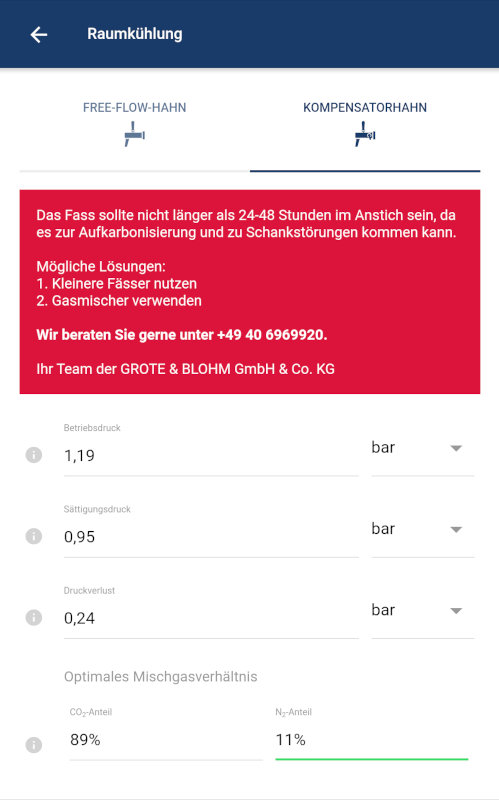
\includegraphics[width=4.8cm]{images/groteblohm.jpg}
\caption{FOBB-APP}
\label{fig:groteblohm}
\end{figure}

Ist eine Zapfanlage korrekt eingestellt, gestaltet sich der Ausschank einfach \autocite{BrewersAssociation2019}: Bierglas im 45° Winkel unter dem Zapfhahn platzieren und den Zapfhahn voll öffnen. Bei halbem Füllstand dann das Bierglas langsam senkrecht aufrichten und den Zapfhahn bei gewünschtem Füllstand schließen. Die Auslauftülle des Hahns sollte dabei nie ins Bier eingetaucht werden. Für höhere Schaumstabilität ist der Zapfvorgang kurz vor Ende zu unterbrechen. Dabei ist das Glas solange abzustellen, bis sich der darin befindliche Schaum leicht gesetzt und gefestigt hat. Danach kann die finale Schaumkrone aufgezapft werden.

Bei längeren Schankpausen erwärmen sich Zapfarmaturen und auch das Bier in den Leitungen. Darüber hinaus sammelt sich Gas im Bereich des Hahns. Dadurch werden mitunter Schankstörungen während der ersten Zapfvorgänge verursacht. Bier, das länger ungekühlt in einer Bierleitung verweilt hat, ist nicht mehr für den Ausschank geeignet. Bei selbst abgefüllten Fässern bildet sich ohne weitere Filtervorgänge gleich wie bei Flaschen ein Hefesatz. Dieser sollte jedoch nach den ersten Zapfvorgängen ausreichend herausgespült sein. \autocite{Krueger2015}

\section*{Kegerator und Keezer}

Mit entsprechenden handwerklichen Fähigkeiten lassen sich (günstige gebrauchte) Kühlgeräte mit vertretbarem Kostenaufwand in Zapfanlagen umrüsten, also Kühlschrank zu Kegerator \cite{Vitaly2019} und Gefriertruhe zu Keezer \autocite{HomebrewAcademy2021}. Auch der Umbau einer (aktiven) Kühlbox zu einer tragbaren Schankanlage bzw. Jockey Box ist eine Option. Die für die Umrüstung benötigten Teile sind auch von Privatpersonen über den Fachhandel zu beziehen.

Bierleitungen können entweder durch eine Gehäusedecke eines Kühlgeräts über eine Schanksäule oder durch Gehäusewände durch einen Durchlaufstutzen an einen Zapfhahn geführt werden. Seiten- und Rückwände enthalten Kühlleitungen. Es ist demnach darauf zu achten, diese nicht bei Bohrungen zu beschädigen. Zur Minimierung von Schankstörungen sollten Bierleitungen zur Gänze im Kühlbereich verlaufen.

Die Umrüstung zum Keezer kann auf nicht destruktive Weise erfolgen. Dazu ist ein Holzaufbau anzufertigen, der zwischen Kühltruhentür und Kühltruhe zu montieren ist. Die Bohrungen für die Durchlaufstutzen erfolgen dann durch diesen Holzaufbau. Bei Gefriergeräten, die keine Einstellung für typische Biertemperaturen besitzen, besteht die Notwendigkeit, eine alternative Temperatursteuerung, wie zum Beispiel einen Inkbird Controller, zu installieren.

\section*{Reinigung und Pflege}

Für Schankanlagen der Gastronomie spezifiziert das österreichische Lebensmittelbuch verschiedene Reinigungsprozeduren/-intervalle. Einige dieser Vorgaben lassen sich auch sinnvoll im Heimbereich anwenden, insbesondere die Reinigung der Zapfhähne mit Wasser und 70 \% Alkoholdesinfektion nach der letzten Verwendung eines Tages. \autocite{BMArbeit2016} Die amerikanische Brewers Association empfiehlt, alle 14 Tage eine chemische Reinigung durchzuführen. Hierbei sind die Bierleitungen zuerst mit einem sauren Reinigungsmittel, dann mit einem alkalischen Reinigungsmittel und danach mit Wasser durchzuspülen. Dies dient der Entfernung von Bierstein und Bakterienansammlungen. Eine Tiefenreinigung aller Kupplungen sollte alle sechs Monate erfolgen und Bierleitungen sind bei erkannter Beschädigung oder spätestens nach zwei Jahren Betriebsdauer zu ersetzen. Darüber hinaus hinterlassen Getränke wie Cider starke aromatische Rückstände in einer Leitung. In diesem Fall ist ebenfalls ein Leitungswechsel zu erwägen. \autocite{BrewersAssociation2019}

Kegs müssen vor dem Öffnen entlüftet werden (Druckabbau). Bei Cornelius Kegs ist dies über einen Zug am Ring des Überdruckventils zu bewerkstelligen. Für Euro Kegs existiert spezielles Werkzeug. Cornelius Kegs lassen sich mit einem Gabelschlüssel zerlegen. Hierzu sind die Gegenstellen für die Kupplungen abzuschrauben. Danach lässt sich das Steigrohr (Degen) herausziehen. Der Ausbau des Überdruckventils erfolgt durch Drehung am Zugring des Ventils. Um die Lebensdauer von Dichtungsringen zu erhöhen, sollten diese mit einem temperaturbeständigen und lebensmittelechten Schmiermittel wie Silikonfett behandelt werden. Hierbei ist allerdings zu beachten, dass Silikonfett bei Kontakt der Schaumstabilität schadet.

\section*{Flaschenabfüllung mit Gegendruckabfüller}

Auch wenn der Großteil des eigenen Biers über eine Zapfanlage ausgeschenkt wird, kann immer noch der Bedarf bestehen, eine kleinere Menge davon in Flaschen abzufüllen. Da Bier in einem Keg aber unter Druck steht und bereits karbonisiert ist, muss der Volumenstrom beim Abfüllen soweit begrenzt werden, dass es in einer Zielflasche nicht zu einer starken Schaumbildung kommt. Das ist bei moderat karbonisierten Bieren mithilfe eines Gegendruckabfüllers (\autoref{fig:gegendruckabfuller}) zu bewerkstelligen.

\begin{figure}[h]
\centering
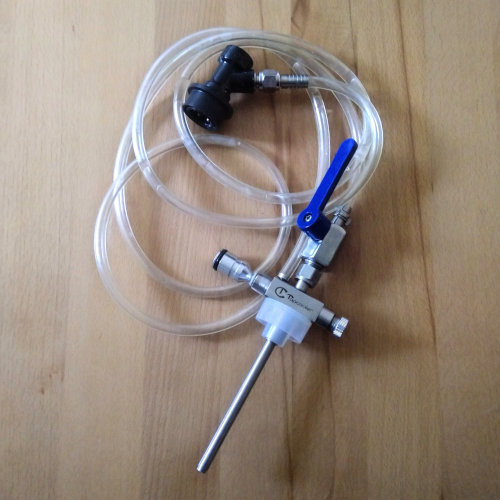
\includegraphics[width=4.8cm]{images/gegendruckabfuller.jpg}
\caption{Tapcooler Gegendruckabfüller mit NC Kupplung}
\label{fig:gegendruckabfuller}
\end{figure}

Von der Konstruktion her ist ein Gegendruckabfüller ein einfaches Gerät. Es besteht aus einem Füllrohr, einem Stopfen, jeweils einem Anschluss und einem Absperrhahn für Bier und \ch{CO2} und einem Auslass mit einem Drosselventil, der als Überlauf dient \autocite{Gretzschel2016}. Teurere Modelle besitzen auch einen durchsichtigen Schutzschild, der u. a. vor Splittern von berstenden Flaschen schützen soll. Zur eigenen Sicherheit wäre ohne Schild zumindest die Verwendung einer Schutzbrille zu empfehlen. Für den Betrieb werden zusätzlich noch eine Bierleitung, zwei Gasleitungen und entweder zwei Druckminderer oder ein Druckminderer mit zwei Ausgängen benötigt. Eine Gasleitung ist hierbei mit dem Keg und eine mit dem Gegendruckabfüller verbunden.

Das Zapfgas hat während der Abfüllung mehrere Aufgaben: Es dient zum Vorspannen der Flaschen, muss den Sättigungsdruck im Keg aufrechterhalten und dient der Förderung. Bier sollte vorab auf eine möglichst tiefe Temperatur abgekühlt werden, damit der Transfer in die Flasche unter möglichst geringem Betriebsdruck erfolgen kann \autocite{Gretzschel2016}. Zur Vermeidung von Schankstörungen ist die Temperatur über den gesamten Abfüllungszeitraum möglichst konstant zu halten.

Für die Abfüllung sind zuerst die Zuleitungen am Gegendruckabfüller zu schließen und das Drosselventil auf eine stärkere Verengung einzustellen. Der Betriebsdruck sollte zumindest so hoch eingestellt werden, dass es zu keiner stärkeren Gasentbindung innerhalb der Bierleitung kommt, also zumindest möglichst nahe am Sättigungsdruck. Dann ist das Füllrohr in eine Flasche einzuführen. Durch ein kurzes Öffnen der Gaszuleitung kann der darin beinhaltende Sauerstoff zum Teil entfernt werden. Danach ist die Flasche mit dem Stopfen zu verschließen und durch erneutes kurzes Öffnen der Gaszuleitung mit \ch{CO2} vorzuspannen. Ist der Druck in der Flasche zu hoch, wird Flüssigkeit zurück ins Keg gedrückt. Ist er zu gering, bildet sich vermehrt Schaum in der Flasche. Abschließend ist die Bierzuleitung noch bis zum gewünschten Füllstand zu öffnen. Der Volumenstrom lässt sich hierbei durch eine Justierung des Drosselventils steuern. Nach dem Schließen der Bierzuleitung kann noch einige Sekunden lang Schaum oder Gas aus dem Überlauf austreten. Um „Bierduschen“ zu vermeiden, sollte währenddessen der Stopfen nicht entfernt werden.

\section*{Kegmenter: Keg als Gärbehälter}

Da Kegs druckbeständig sind, lassen sie sich bei geringerem Füllstand auch für die Druckvergärung zweckentfremden. Egal ob drucklose Gärung oder Gärung unter Druck, grundsätzlich muss in beiden Fällen sichergestellt sein, dass Überdruck entweichen kann. Dies kann entweder über eine aufgesteckte Kupplung, ein geöffnetes Spundventil oder durch einen Spunddruckregler (\autoref{fig:spundapparat}) erfolgen. Für eine möglichst trubarme Bierentnahme nach der Gärung kann in einem Keg ein schwimmendes Tauchrohr installiert werden. \autocite{Felmann2020}

\begin{figure}[h]
\centering
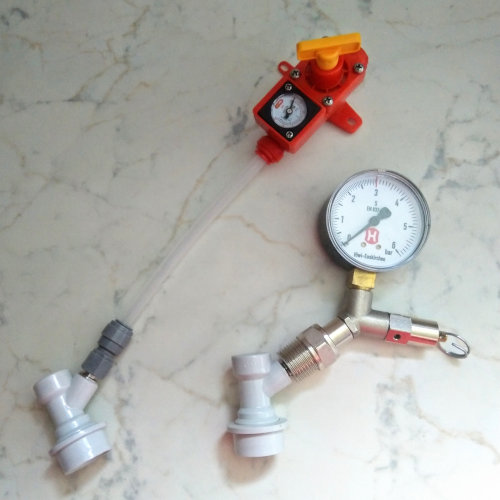
\includegraphics[width=4.8cm]{images/spundapparat.jpg}
\caption{Spunddruckregler mit NC Kupplung}
\label{fig:spundapparat}
\end{figure}

Spunddruckregler lassen sich auf einen Maximaldruck einstellen. Gängige Empfehlungen im Heimbraubereich hierfür sind 0,35 bis 0,7 Bar. Wird dieser Druck überschritten, öffnet sich das integrierte Ventil und baut somit den Überdruck ab. Nicht jeder Regler verfügt über eine Einstellschraube mit Skala. Ist keine Skala vorhanden, kann die Einstellung mithilfe eines Kegs bestimmt werden. Hierzu ist mittels eines Druckminderers der gewünschte Druck im Keg aufzubauen. Der Spunddruckregler wird auf den höchstmöglichen Druck eingestellt und mit der Einstellschraube solange justiert, bis \ch{CO2} aus dem Ventil zu entweichen beginnt.

\section*{Zusammenfassung}

Die revanten Eckpunkte dieses Artikels sind:

\begin{itemize}
\item Eine minimale Zapfanlage besteht aus einem Keg, einem Druckgasbehälter und einer Zapfarmatur. Alle Anschlüsse erfolgen direkt an das Keg mittels Kupplung bzw. Zapfkopf.

\item Gängige Kegtypen im Heimbraubereich sind Cornelius NC Kegs und Euro/DIN Kegs.

\item Die Karbonisierung lässt sich gleich wie bei der Flaschengärung oder durch Zwangskarbonisierung bei spezifischem Sättigungsdruck durchführen.

\item Der Druck in einem Keg kann mit einem Spundventil gemessen und reduziert werden.

\item Die Abfüllung von einem Gärbehälter aus erfolgt wie gewohnt durch Umschlauchen. Aus Druck-Gärbehältern ist ein geschlossener Transfer mit minimaler Sauerstoffeinwirkung möglich.

\item Ein störungsfreier Ausschank erfordert eine gut ausbalancierte Zapfanlage mit einem korrekt eingestellten Betriebsdruck. Kompensatorhähne können hierbei Störungen bis zu einem gewissen Grad ausgleichen. Ein zu hoher Betriebsdruck führt bei reiner \ch{CO2} Zuführung zur Überkarbonisierung.

\item Zapfanlagen verursachen einen kontinuierlichen Reinigungsaufwand.

\item Die Flaschenabfüllung aus einem Keg ist mit einem Gegendruckabfüller zu bewerkstelligen.

\item Kegs lassen sich in Verbindung mit einem Spunddruckregler als Druck-Gärbehälter einsetzen.
\end{itemize}

Weiterführende Informationen zum Aufbau und Betrieb von Schankanlagen können der spezifischen Fachliteratur entnommen werden. Der deutsche Brauer-Bund bietet in diesem Bereich den kostenpflichtigen  „\href{https://brauer-bund.de/shop/leitfaden-getraenkeschankanlagen}{Leitfaden Getränkeschankanlagen}“ an. 

\printbibliography[title=Quellen]

\end{document}